\section{Analysemuster}

\begin{tcolorbox}[title=Analysemuster]
    Im Software Engineering versteht man unter dem Begriff \textit{Muster} (\textit{Pattern}) \textbf{vorgefertigte Lösungsschablonen für verallgemeinerte Probleme}.\\
    Die Beschreibung der verallgemeinerten Probleme und Lösungen auf eine \textbf{formalisierte Weise} nennt man \textbf{Muster}.\\
    Muster müssen zur Anwendung auf ein konkretes Problem \textit{konkretisiert} werden.\\
    Im Bereich des Software Engineerings gibt es Muster für \textbf{Analyse}, \textbf{Architektur}, \textbf{Entwurf}.\\

    \noindent
    \textbf{Vorteile}:
    \begin{itemize}
        \item es stehen \textbf{bewährte Standardlösungen} zur Verfügung
        \item Verwendung bereits bewährter Lösungen ist oft \textbf{schneller und besser} als selbstentwickelte neue Lösungen
        \item Muster helfen bei der \textbf{Kommunikation}
    \end{itemize}
\end{tcolorbox}

\begin{tcolorbox}[title=Beispiele]
    \begin{itemize}
        \item \textbf{Exemplartyp} (Abstraction-Occurence): Objekte einer Klasse ähneln sich untereinander und tragen gemeinsamen, gleiche Informationen oder besitzen gleiches  Verhalten, unterscheiden sich aber wesentlich
        \item \textbf{Wechselnde Rollen} (Player-Role): ein Objekt kann in unterschiedlichen Kontexten verschiedene Verantwortlichkeiten und Beziehungen haben
        \item \textbf{Allgemeine Hierarchie} (General Hierarchy, Kompositum): Objekte können hierarchisch angeordnet sein;
         jedes Objekt kann maximal einem Objekt untergeordnet sein;
         manche Objekte dieser Hierarchie können keine untergeordneten Objekte haben
    \end{itemize}
\end{tcolorbox}

\begin{figure}
    \centering
    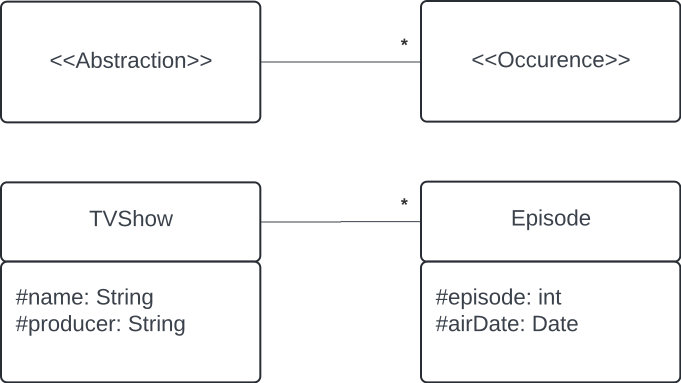
\includegraphics[scale=0.3]{part two/Objektorientierte Analyse/img/abstractionoccurence}
    \caption{Beispiel für das \textit{Abstraction-Occurence-Pattern}. (Quelle: eigene)}
    \label{fig:abstractionoccurence_cc}
\end{figure}
\begin{figure}
    \centering
    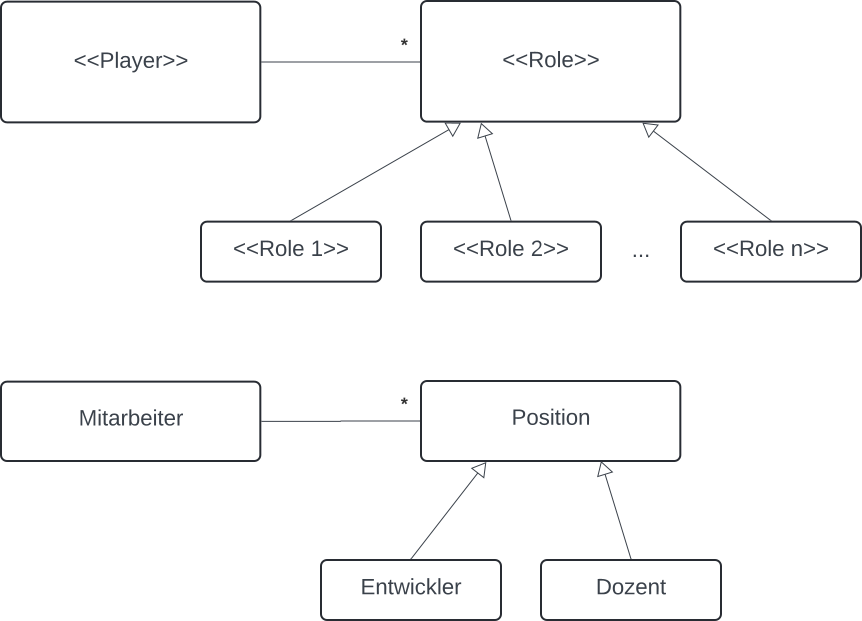
\includegraphics[scale=0.3]{part two/Objektorientierte Analyse/img/playerrole}
    \caption{Beispiel für das \textit{Player-Role-Pattern}. (Quelle: eigene)}
    \label{fig:playerrole_cc}
\end{figure}
\begin{figure}
    \centering
    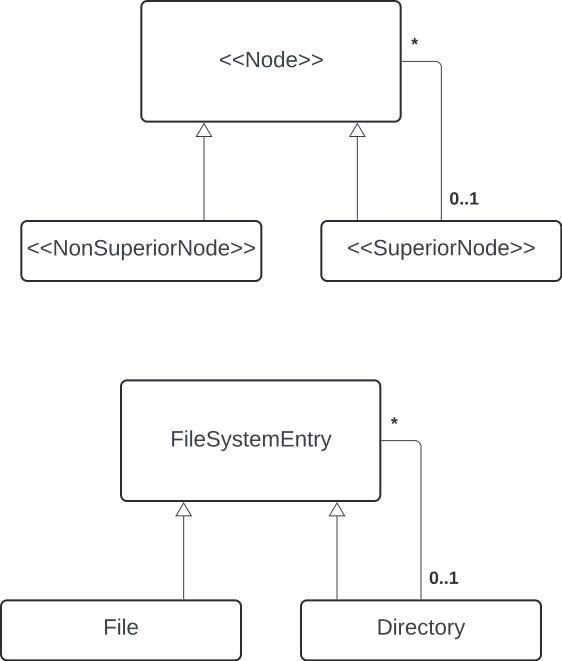
\includegraphics[scale=0.3]{part two/Objektorientierte Analyse/img/generalhierarchy}
    \caption{Beispiel für das \textit{General-Hierarchy-Pattern}. (Quelle: eigene)}
    \label{fig:generalhierarchy_cc}
\end{figure}